\chapter{Background}
\label{c:background}

\section{Modern vehicles}

In recent years, vehicles have become ever smarter, providing functionality that goes beyond simple transportation of passengers and goods. They can guide us through \gls{gps}, make calls, receive over-the-air updates, inform other vehicles of their position, and even drive themselves. Having this computational capacity, being identifiable, able to transfer data over a network and connected to each other makes modern vehicles a part of the \acrlong{iot} \citep{Lombardi2021}.\par

\subsection{Architecture}

An overview of the architecture of a modern vehicle can be seen in Figure \ref{fig:Car_Domains}. It is common practice to have several domains connected by a central gateway \gls{ecu}.

\begin{figure}
    \centering
    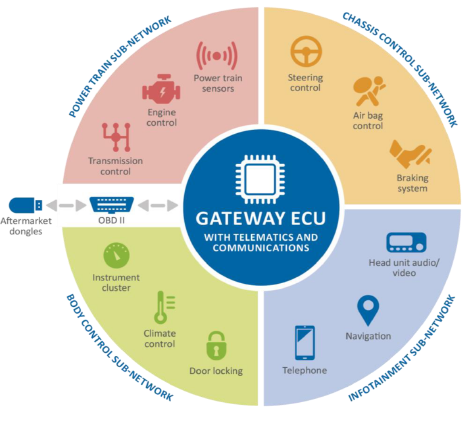
\includegraphics[width = .7\textwidth]{img/parts/introduction/Vehicle Architecture.png}
    \caption{Main domains of a modern car \citep{ENISA}}
    \label{fig:Car_Domains}
\end{figure}

In all of these domains, \glspl{ecu} are responsible for controlling their components, such as precise fuel combustion in the powertrain domain or air conditioning in the body control domain. These controllers are often based on the ARM platform, with an automotive-grade product line generally being used due to unique constraints in the automotive environment.\par

In 2003, the \gls{autosar} was established as a "worldwide development partnership of vehicle manufacturers, suppliers, service providers and companies from the automotive electronics, semiconductor and software industry" with the objective of creating an open and standardised software architecture for \gls{ecu}. The use of such a manufacturer independent standard allows for a reduction in development effort and improved software quality, as software modules can be used in vehicles of different manufacturers and components of suppliers, thereby reducing complexity and expense. \gls{autosar} maintains five standards: the \gls{autosar} Classic Platform, the \gls{autosar} Adaptive Platform, the Foundation, \gls{autosar} acceptance tests, and \gls{autosar} application interfaces.\par

The \gls{autosar} Classic architecture is shown in Figure \ref{fig:autosar_arch}. It is composed of three software layers which run on a microcontroller: application, \gls{rte}, and \gls{bsw}. The \gls{rte} handles communication between the application layer, which is mostly hardware independent, and the \gls{bsw}. The \gls{bsw} is then divided intro three layers, along with complex drivers: services, \gls{ecu} abstraction, and microcontroller abstraction. Services are divided further, into functional groups representing the infrastructure for system, memory and communication services.

\begin{figure}
    \centering
    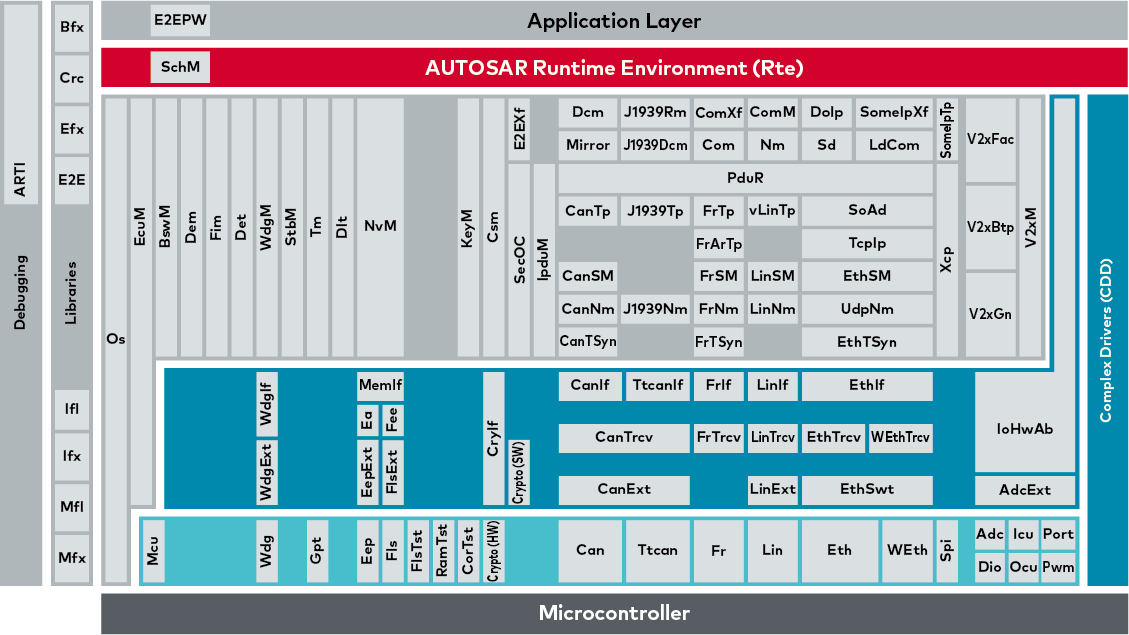
\includegraphics[width = \linewidth]{img/parts/introduction/AUTOSAR.png}
    \caption{The \gls{autosar} architecture \citep{autosar_arch}}
    \label{fig:autosar_arch}
\end{figure}

The \gls{vfb} allows for communication between different \glspl{swc} and the use of \gls{bsw} services, both within the individual \gls{ecu} and between \glspl{ecu}. Because the development of \glspl{swc} is based on the \gls{vfb}, \glspl{swc} are independent of the underlying hardware, making them easier to reuse and integrate into different projects on different platforms as well as to flexibly relocate existing \glspl{swc} to \glspl{ecu} during development.\par

New use cases, such as autonomous driving, communication with traffic infrastructure, multimedia applications, and smartphone integration, led to the creation of the \gls{autosar} Adaptive Platform. This standard aims to provide support for the deployment of customer applications and an environment for applications that require a high amount of computing power (\textit{e.g.} computer vision). It implements the \gls{autosar} Runtime for Adaptive Applications, with a POSIX-based operating system at its core running \citep{autosar_adaptive_os} on virtualized hardware. In contrast to the \gls{autosar} Classic Platform, the \gls{autosar} Runtime Environment for the Adaptive Platform dynamically links services and clients during runtime. This allows applications to be developed, tested and distributed or updated independently of one another.

\begin{figure}
    \centering
    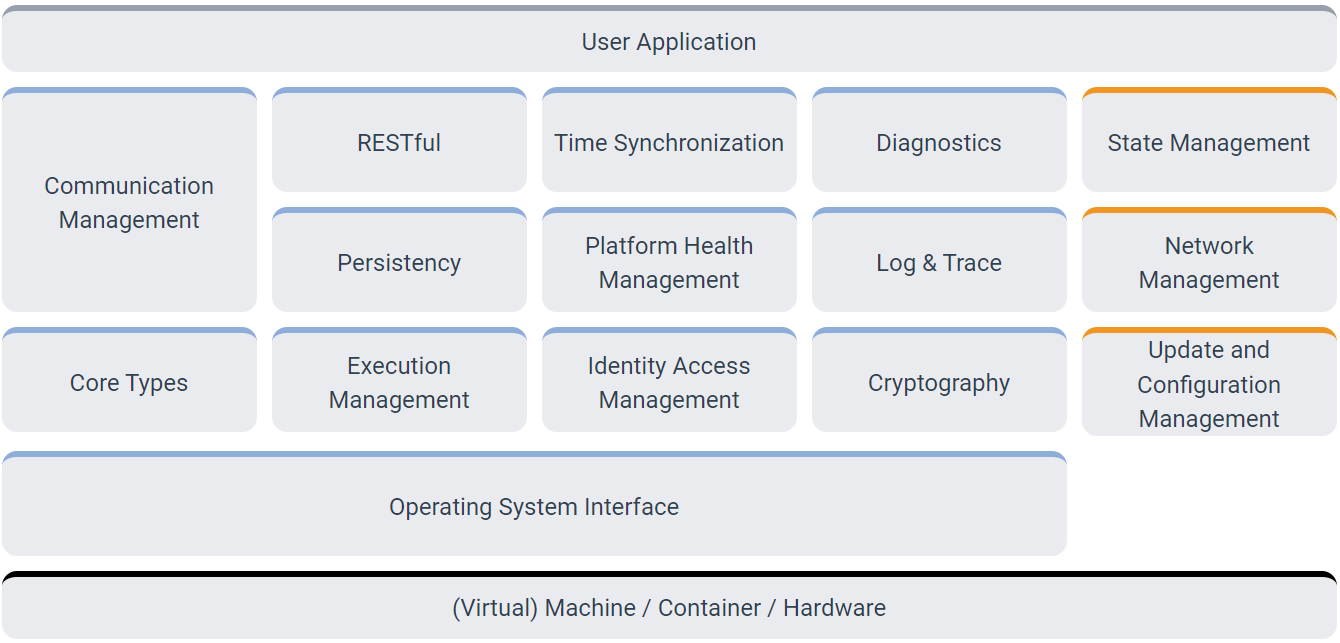
\includegraphics[width = \linewidth]{img/parts/introduction/AUTOSAR Adaptive Platform.png}
    \caption{The \gls{autosar} Adaptive Platform architecture \citep{autosar_adaptive_arch}}
    \label{fig:autosar_adaptive_arch}
\end{figure}

The Foundation standard enforces interoperability between the \gls{autosar} platforms by the means of common requirements and technical specifications shared between the \gls{autosar} platforms, \textit{e.g} bus protocols and common aspects of the methodology.\par

Acceptance Tests for Classic Platform are system tests that validate \gls{autosar} stack behaviour at the bus and application level. \gls{autosar} provides tests that cover \gls{rte} requirements, \gls{bsw} services, and bus protocols and behaviour. It also allows for the addition of tests by the user to certify specific features not covered in the standard set.\par

The Application Interfaces standard covers syntax and semantics for the body and confort, powertrain engine, powertrain transmission, chassis control, ocupant and pedestrian safety, and human-machine interface, multimedia and telematics domains. The deployment of standardised application interfaces assures software reusability independently of specific hardware and/or \glspl{ecu}, which is one of the main requirements of \gls{autosar}.

\subsection{Applications}

A significant part of automotive innovation has been driven by software applications. These take advantage not only of the data generated by internal sensors to perform complex tasks but allow for better multimedia functionality and communication with external entities. In \cite{Le2018}, the authors state that automotive applications can be classified based on these 5 criteria: functional domain, influence on safety, driver involvement, connectivity, and time constraint.\par

Applications like the anti-lock braking system are real-time functional and safety-critical systems with no driver involvement or external connectivity elements. Another safety-critical application is adaptive cruise control, which is part of the \gls{adas} class of applications. However, unlike the anti-lock braking system, it requires some level of awareness from the driver. A network application like door and window control via smartphone is real-time and interacts with the vehicle’s body.\par

Such an increase in computational complexity allows for the introduction of vulnerabilities in the software and, with applications extending multiple domains and interacting with other applications, there is an increased concern about their security. Until recently, applications were developed by the manufacturers to run directly on the embedded hardware. The usual approach was to add a new \gls{ecu} for every new function to be implemented. However, this method has made the vehicle’s internal network too complex for safe and efficient handling. Therefore, a platform-based approach has become of interest to both manufacturers and developers as it provides developers with an abstraction of the underlying hardware as well as making it possible to write reusable applications to run on the same standardised platform, but different hardware. This simplifies both the application development as well as its deployment. Besides, the authors in \cite{Holle} suggest that an approach like that of the mobile platforms could be taken. In this case, an open \gls{sdk} is provided to third-party developers to create and distribute their applications similarly to mobile app stores.\par

This increase in application diversity and functionality means that the vehicle handles much more sensitive information, especially when considering its connectivity to devices as personal as one’s smartphone. This includes information like common routes and schedules, call history, or even conversations recorded with the internal microphones (otherwise used for phone conversations on virtual assistances). As such, modern vehicles are becoming a major target for attackers who seek to obtain information on the user, not only because they contain sensitive information, but also because of the lack of security elements present in the vehicle design and architecture. This is because manufacturers have always designed their vehicles with safety, but no security in mind \citep{Siegel2018}.

\section{Engineering Standards}

Functional safety is already an integral part of road vehicle engineering, with the functional safety norm \cite{ISO26262} being well established. The industry's pursuit to design and build safer connected vehicles is leading to the development of several secure software development standards for the automotive sector. One such standard is the \cite{ISO21434} Road Vehicles - Cybersecurity Engineering. It's predecessor, \cite{SAEJ3061}, already established some high-level guiding principles such as defining a complete lifecycle process framework, and it also recommends an initial assessment of potential threats and risks that may be considered relevant.\par

An overview of the ISO/SAE 21434:2021 can be found on Figure \ref{fig:iso21434toc}. Clause 4 offers some general considerations and contextualises the approach to vehicle cybersecurity taken in the standard. Clause 5 concerns the organisational structure, and describes the organisation's security objectives and how to achieve those objectives as well as responsibility and authority assignment. Clause 6 discusses cybersecurity management at the project level, detailing, among others, the proposed approach for tailoring and incorporating off-the-shelf components. Clause 7 describes cybersecurity responsibility distribution between customer and supplier. Clause 8 details the continuous development activities, such as risk assessment and vulnerability management, until the end of cybersecurity support. Clause 9 concerns the concept phase, which involves considerations of vehicle functionality as well as the cybersecurity goals for each item. Clauses 10 and 11 discuss the product development phase, including the specification of cybersecurity requirements and architectural design, as well as integration and verification activities and the validation of cybersecurity goals and claims. Clauses 12 to 14 describe the components of the post-development phase, such as production (manufacturing and assembly of an item or component), operations and maintenance (including cybersecurity incident response), and end of support and decommissioning. Finally, Clause 15 discusses threat analysis and cybersecurity risk assessment.

\begin{figure}
    \centering
    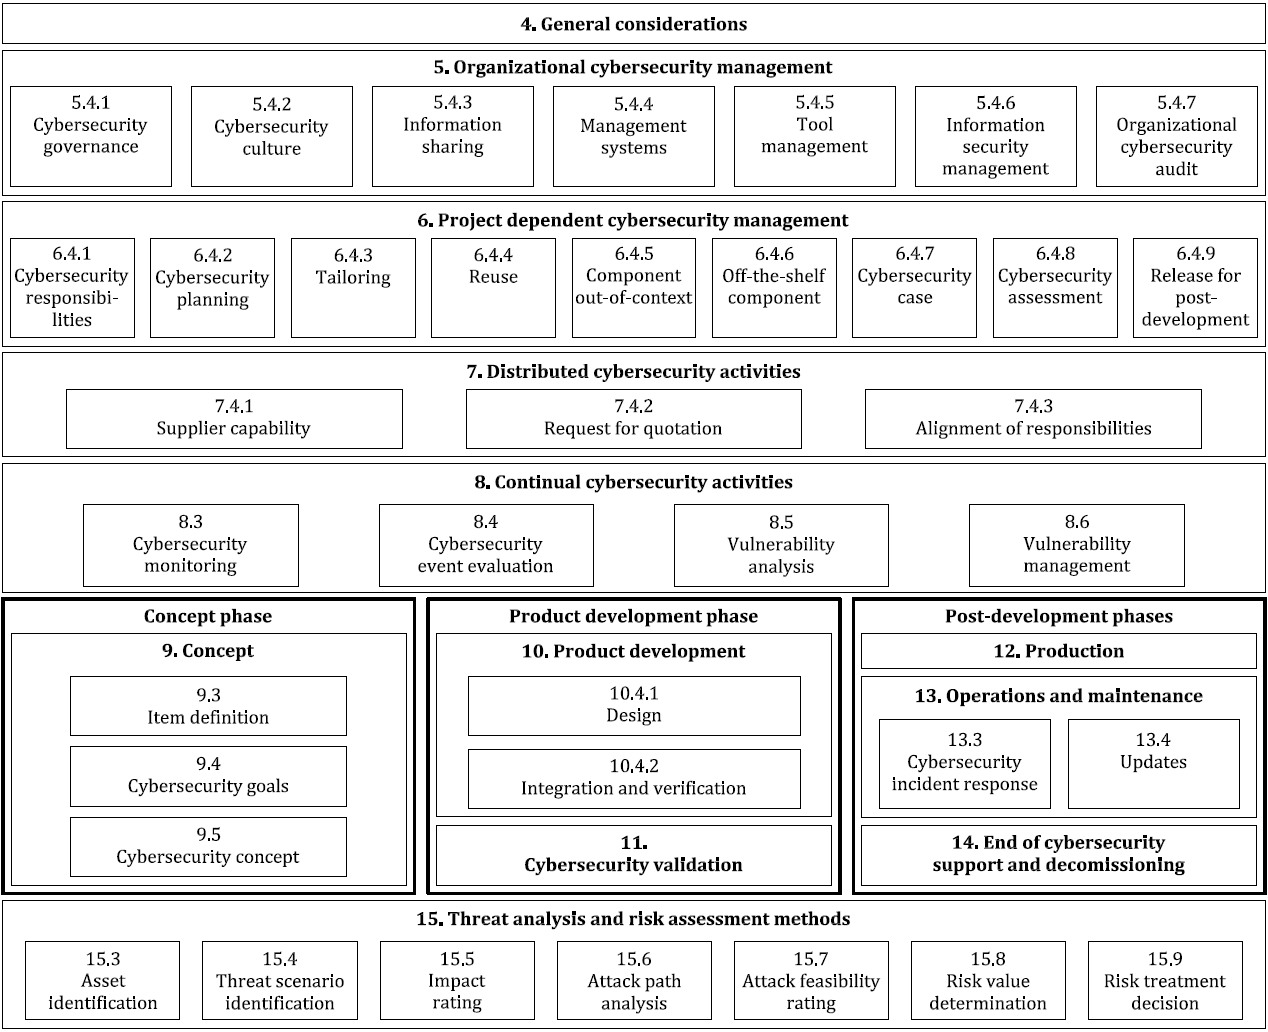
\includegraphics[width = \textwidth]{img/parts/introduction/ISO 21434 ToC.png}
    \caption{Content overview of the \cite{ISO21434}}
    \label{fig:iso21434toc}
\end{figure}

\section{In-vehicle networks}

For a long time, the only electronic component in a vehicle was the radio. However, pushes for more environmentally friendly vehicles, as well as increased comfort, led to the addition of many more electronic modules. These can be a part of several subsystems, such as the powertrain, chassis, body, and infotainment system, each with its own set of requirements. These requirements may be an assurance of message delivery and minimum delivery times for safety-critical applications, or high bandwidth for infotainment purposes. Longevity must also be considered. In \cite{AvgCarAge}, it was shown that the average car age in the European Union is 11.5 years. For comparison, the average smartphone lifespan for consumers in the United States has been documented to be around 2.75 years \citep{AvgPhoneAge}. Network boot-time is relevant as well, as automotive boot-time should remain under 100ms, while some smartphones take over 1 minute to boot \citep{AutomotiveNetworks}. Power consumption must not be forgotten, as it impacts the vehicle's range. The manufacturer's desire to reduce the vehicle's complexity, weight, and cost, led to the use of a heterogeneous set of networks with different characteristics.\par

\cite{AutomotiveNetworks} lists some roles that a network might serve. These are safe/time-critical data, control data, backbone, infotainment, multi-gig data, and low cost/speed data. Below is an introduction to some of the dominant automotive network protocols, and a general overview of these networks can be seen in Table \ref{fig:auto_networks}.

\begin{table}
    \centering
    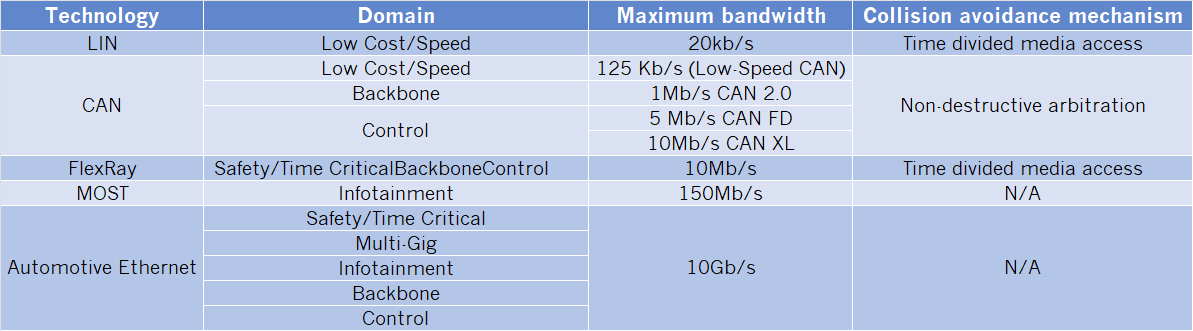
\includegraphics[width = \textwidth]{img/parts/introduction/Network Table.png}
    \caption{Characteristics of dominant automotive networks}
    \label{fig:auto_networks}
\end{table}

\subsection{Controller Area Network}
\label{subsec:can}

The development of the \gls{can} standard was started in 1983 by Uwe Kiencke. It was first introduced in February of 1986 at the Society of Automotive Engineers Congress by Robert Bosch GmbH \citep{can}. Following the publication of \gls{can} 2.0 by Bosch in 1991, the \gls{iso} released the \gls{can} standard ISO 11898. The Mercedes W140, first available in 1991, was the first vehicle with a \gls{can}-based in-vehicle network \citep{CAN_Merc}.\par

\gls{can} messages are sent in broadcast mode, which means that all \glspl{ecu} in a network receive all transmissions. Devices that receive a message acknowledge their reception. Each \gls{ecu} listens for messages from a subset of IDs, and each message ID must be sent by no more than one \gls{ecu} \citep{kulandaivel2019canvas}. It was designed with the objective of building a low-cost, and reliable network, and is therefore used mainly used for powertrain, chassis and body electronics. Its limited bandwidth of 1Mb/s does not allow for its use in other domains, such as the infotainment system \citep{Huang2019}.\par

A deeper look into \gls{can} is conducted in Section \ref{s:can}.

\subsection{Local Interconnect Network}

\gls{lin} is a supplement to the \gls{can} bus, offering lower performance and reliability, but also a much lower cost. It is a product of the \gls{lin} Consortium, founded by BMW, Volkswagen Group, Audi, Volvo Cars Mercedes-Benz, Volcano Automotive Group, and Motorola, and provides cost-efficient communication in applications where the bandwidth and versatility of \gls{can} are not required. This typically includes mechatronic nodes like the vehicle’s windows, wipers, side mirrors, or seat controllers \citep{LIN}.\par

The first version of the specification was released in 1999, with updates soon following. \gls{lin} 2.0 was released in 2003 and the protocol was standardised in ISO 17987:2016.\par

Unlike \gls{can}, a typical \gls{lin} cluster consists of a single commander node and up to 16 responders connected by a single copper wire, with communication speeds up to 20kbit/s \citep{Takahashi2017}. It is usually deployed as a \gls{can} sub-network, with only the \gls{lin} master node being connected to the \gls{can}-bus. All communications are initiated by the commander node, with one responder replying to a given message identifier (the commander node can also act as a responder, replying to its own messages). There is, therefore, no need to implement collision detection \citep{LIN_CSS}.\par

This protocol also implements a sleep and wake-up mechanism, allowing it to potentially save power. Responders can enter sleep via a command issued by the commander node or are forced into that state after more than 4 seconds of \gls{lin} inactivity. The wake-up command can be issued by any node \citep{LIN}.
We can see in Figure \ref{fig:auto_nodes} that the number of \gls{lin} nodes has recently surpassed the number of \gls{can} nodes.

\begin{figure}
    \centering
    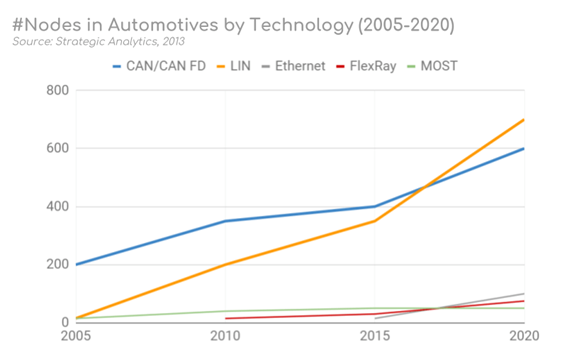
\includegraphics{img/parts/introduction/LIN Nodes.png}
    \caption{Number of nodes in automotive by technology \citep{LIN_CSS}}
    \label{fig:auto_nodes}
\end{figure}

There have been recent efforts to study the security aspects of \gls{lin}, such as the one detailed in \citep{Takahashi2017}, and it is noted that due to its link with \gls{can}, the latter’s vulnerabilities are also a cause for concern for the former. \citep{Ernst2018} showed that a compromised \gls{lin} node can destroy as well as create "erroneous, but valid packets". The authors also suggested that the effect of an intrusion can be minimised by the use of appropriate firewalls. However, since \gls{lin} is usually used for non-safety-critical purposes, compromising the bus would most likely not be life-threatening.

\subsection{FlexRay}

The continuous search for improved safety, performance, and comfort of vehicles means that the speed and reliability of data communicated between \glspl{ecu} must increase. FlexRay was developed by the FlexRay Consortium, founded in 2000 by Daimler Chrysler and BMW along with Motorola and Phillips, and disbanded in 2009. The Consortium had the goal of creating a bus protocol capable of delivering achieving high data rate, deterministic and fault-tolerant communications \citep{FlexRayFreescale} as a way of overcoming \gls{can}'s limitations in these aspects. Features that require a higher throughput for safety/time-critical data like active cruise control, anti-lock braking system, or break-by-wire, thus use FlexRay as the preferred communication protocol, as it satisfies the reliability requirements for these safety-critical systems.\par

The FlexRay bus consists of a single twisted-pair copper cable, with \glspl{ecu} connected using multi-drop technology. Its clock synchronisation is deterministic and uses time divided media access as a collision avoidance mechanism, in contrast to the arbitration mechanism used by \gls{can}. This makes it suitable for safety/time-critical applications. It is also used for backbone and control data, similarly to \gls{can}. However, it provides much higher bandwidth: 10Mb/s, compared to \gls{can}'s maximum of 1Mb/s, and is more expensive \citep{Huang2019}.\par

The protocol is defined in \gls{iso} 17458-1 to 17458-5.

\subsection{Media Oriented Systems Transport}

As the name suggests, \gls{most} is primarily used for high-speed multimedia. It can use either a single twisted pair of copper cables, or plastic optical fibre (which has the advantage of being completely immune to electromagnetic disturbance), and supports 25, 50, and 150 Mb/s data transfer speeds \citep{MOSTMicrochip}. The \gls{most} network is capable of managing up to 64 devices, usually configured in a ring topology. Star or double ring configurations are also possible \citep{MOSTVector}, with the latter being relevant for safety-critical applications \citep{Huang2019}.\par

The \gls{most} specification, described in ISO 21806, defines the physical and data link layers, as well as all the seven layers of the \gls{iso}/OSI model.

\subsection{Automotive Ethernet}

Automotive Ethernet is an adaptation of standard Ethernet that fulfils the requirements of the automotive environment, such as the use of a single twisted-pair wiring, which provides lower cost and better electromagnetic compatibility.\par

The motivation behind this adaptation is primarily the amount of full-duplex bandwidth it provides. In 2020, IEEE published the IEEE 802.3ch-2020 standard, detailing the specification for automotive Ethernet with data transfer speeds of up to 10Gb/s (10GBASE-T1). This allows fields like \gls{adas} to grow and develop without much concern for bandwidth restrictions. Another important factor is that Ethernet is already an established technology outside of the automotive industry. This means that there is a large knowledge base to support it, especially when compared to the other protocols discussed here. Its use of the IP stack is a point in its favour as well. It is also a scalable technology, with adding new nodes to the network being a relatively easy task \citep{Bello2011}.\par

As for the network topology, Ethernet is, by nature, a point-to-point network. This means that connecting more than two nodes requires an Ethernet switch.\par

This technology does not aim, however, to only replace other high-bandwidth networks like \gls{most}. The 10BASE-T1s version of the automotive Ethernet protocol is a direct competitor to \gls{can} and FlexRay, as it describes a multi-drop bus topology network over a single twisted pair of copper wires with speeds up to 10Mb/s and time divided media access for collision avoidance \citep{AutomotiveNetworks}. This would allow for a vehicle using only IP based technologies, simplifying the overall design of the network.

\section{Controller Area Network}
\label{s:can}

\gls{can} is currently the dominant network protocol in automotive. As laid out in \ref{subsec:can}, it is a broadcast network with no central bus master, which allows for data consistency across the entire system. The two lowest layers of the ISO/OSI model for \gls{can} are defined in the ISO 11898 \citep{Richards2002} and the implementation can be seen in Figure \ref{fig:CAN_ISO}. Protocols such as the CANopen protocol, supported by the \emph{CAN in Automation} group (CiA), establish the link between the physical and data link layers and those above \citep{Corrigan2002}.

\begin{figure}
    \centering
    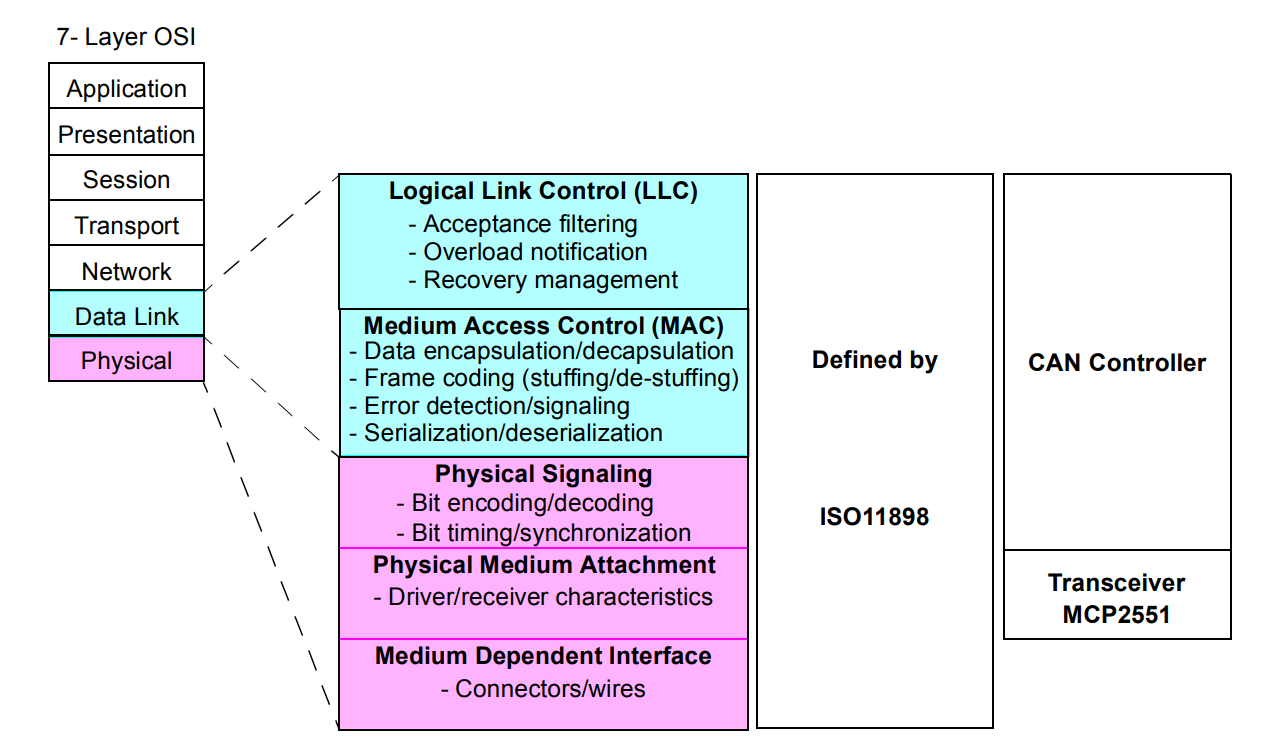
\includegraphics[width = \textwidth]{img/parts/introduction/CAN ISO.png}
    \caption{\gls{can} and the OSI model \citep{Richards2002}}
    \label{fig:CAN_ISO}
\end{figure}

The \gls{can} bus differs from a conventional bus because it inverts the logic state between the bus, driver input and receiver output. In \gls{can}, a logic high is associated with a 0 (the dominant bit), and a logic low with a 1 (the recessive bit) \citep{Corrigan2002}. An illustration of this mechanism can be seen in Figure \ref{fig:CAN_Bus_Logic}.

\begin{figure}
    \centering
    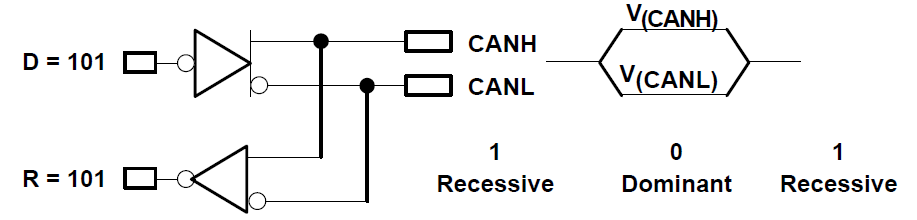
\includegraphics[width = \textwidth]{img/parts/introduction/CAN Bus Logic.png}
    \caption{The inverted logic of a \gls{can} bus \citep{Corrigan2002}}
    \label{fig:CAN_Bus_Logic}
\end{figure}

\gls{can} uses \gls{csma}, meaning that each node must wait for bus inactivity before transmitting, with \gls{cdamp}, meaning that collisions are resolved through bit-wise arbitration using the message's ID field. Messages with lower ID have a higher priority, as a smaller identifier will hold the dominant state on the bus for longer \citep{Corrigan2002}. The bus can, therefore, be thought of as acting as an AND gate, as explained by \cite{Cook2008}.\par

There are four message types in \gls{can}: the data frame, the remote frame, the error frame, and the overload frame. Error-free messages have the last bit of the EOF set as recessive, and a dominant bit in this field causes the message to be re-transmitted.\par

The data frame is the most common message type and is composed of seven fields: SOF, arbitration, control, data, CRC, ACK, and EOF. The SOF field consists of a single dominant bit, and the arbitration decides which of the nodes attempting to transmit is allowed to do so. The RTR field distinguished between data (dominant bit) and remote (recessive bit) frames. The control field indicates the amount of data being sent in the data field. The remote frame is used to request a data frame from another node. If a node broadcasts a remote frame containing a particular identifier, the node responsible for this identifier immediately generates a data frame as a response. The error frame is used to notify errors in frame transmission, and the overload frame signals that the controller has not finished processing the current message, and delays the start of the next message \citep{lee2017otids}.
\gls{can} is available in three generations: Classical \gls{can}, \gls{can} FD, and \gls{can} XL. These are described below.

\subsection{Classical CAN}

There are three versions of what can be called "classical" \gls{can}: low-speed \gls{can}, \gls{can} 2.0A, and \gls{can} 2.0B. As the name suggests, low-speed \gls{can} has limited bandwidth, at 125Kb/s. However, it is fault-tolerant, as it can operate even when one of the two wires fails. This version of the protocol is standardised in ISO 11898-3. \gls{can} 2.0 versions A and B allow for speeds up to 1Mb/s, with the main difference between the two versions being that the former uses an 11-bit identifier (standard), and the latter a 29-bit identifier (extended). The bit fields for standard (low-speed \gls{can} and \gls{can} 2.0A) and extended (\gls{can} 2.0B) versions can be seen of Figures \ref{fig:standard_can} and \ref{fig:extended_can}, respectively. The meaning of the bit fields are:

\begin{itemize}
    \item \textbf{SOF (Start Of Frame)}: Single dominant bit that marks the start of a message.
    \item \textbf{Identifier}: Establishes the priority of a message (lower ID means higher priority).
    \item \textbf{RTR (Remote Transmission Request)}: When this bit is dominant, information is required from the node specified in the identifier.
    \item \textbf{SRR (Substitute Remote Request)}: Replaces the RTR bit as a placeholder in the extended format.
    \item \textbf{IDE (Identifier Extension)}: When this bit is dominant, a standard \gls{can} identifier is being transmitted.
    \item \textbf{r0}: Reserved bit.
    \item \textbf{r1}: Reserved bit.
    \item \textbf{DLC (Data Length Code)}: 4-bit field that contains the number of bytes of data being transmitted.
    \item \textbf{Data}: Up to 64 bits may be transmitted.
    \item \textbf{CRC (Cyclic Redundancy Check)}: 16-bit field containing the checksum of the transmitted data for error detection.
    \item \textbf{ACK (Acknowledge)}: Every accurate message received has this recessive bit overwritten by a dominant bit.
    \item \textbf{EOF (End-Of-Frame)}: 7-bit field that signals the end of a \gls{can} frame, while also disabling bit-stuffing.
    \item \textbf{IFS (Inter-Frame Space)}: 7-bit field that allows the controller enough time to move the received frame into the message buffer.
\end{itemize}

\begin{figure}
    \centering
    \begin{subfigure}{\textwidth}
        \centering
        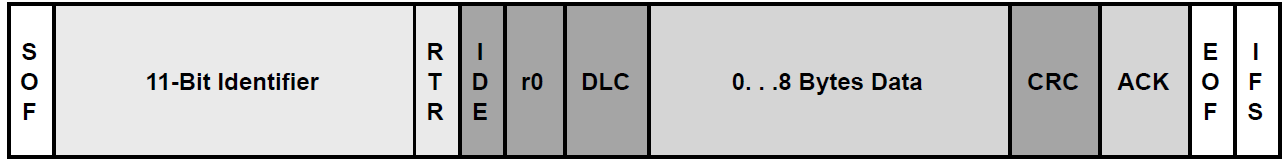
\includegraphics[width=\textwidth]{img/parts/introduction/Standard CAN.png}
        \caption{Standard \gls{can}: 11-bit identifier}
        \label{fig:standard_can}
    \end{subfigure}
    \begin{subfigure}{\textwidth}
        \centering
        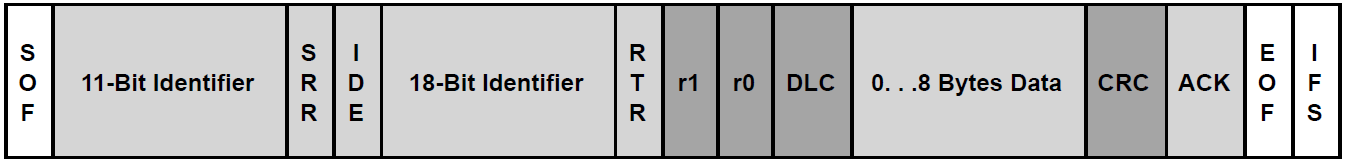
\includegraphics[width=\textwidth]{img/parts/introduction/Extended CAN.png}
        \caption{Extended \gls{can}: 29-bit identifier}
        \label{fig:extended_can}
    \end{subfigure}
    \caption{Classical \gls{can} frame structure \citep{Corrigan2002}}
\end{figure}

\subsection{CAN FD}

Increasing demand for more bandwidth led to the development of \gls{can} FD (standing for Flexible Data-Rate), which was started in 2011 by Robert Bosch GmbH. The fact that this design is based on \gls{can} 2.0 provides several advantages. Costs are similar, and it has a small impact on current software and applications. The physical layer and topologies can also be maintained \citep{Woo2016}. It is primarily used in high-performance vehicle \glspl{ecu} and is established as an international standard in ISO 11898-2:2015.\par

The main difference between \gls{can} 2.0 and \gls{can} FD is the flexible data rate that \gls{can} FD offers. This means that it allows for the data frame to be transmitted at different speeds, depending on the characteristics of the network. Development was faced with two main challenges: avoiding increased message delays caused by placing more bytes of data in a single frame, and maintaining \gls{can}'s practical wiring \citep{CANFD}. The solution to this was the introduction of a new frame structure, which can be seen in Figure \ref{fig:CANFD_Frame}.

\begin{figure}
    \centering
    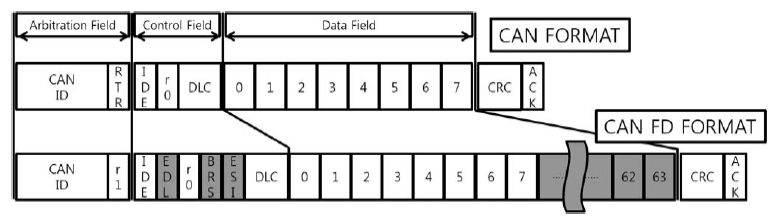
\includegraphics[width = \textwidth]{img/parts/introduction/CAN FD.png}
    \caption{Comparison of \gls{can} and \gls{can} FD data frames \citep{Woo2016}}
    \label{fig:CANFD_Frame}
\end{figure}

In the arbitration field, we can see that the RTR bit is not present in the \gls{can} FD frame. This is because there are no remote frames in \gls{can} FD.\par

Three new bits were added to the control field: extended data length (EDL), bit rate switch (BRS), and error state indicator (ESI). The EDL bit is used to distinguish between the classical \gls{can} (bit is dominant) and the \gls{can} FD (bit is recessive) frame formats. If the BRS bit is dominant, it signals that the data frame is sent at the arbitration rate (i.e. up to 1Mb/s). Otherwise, the remaining part of the data frame is sent at a higher speed (around 5Mb/s). The ESI bit is used for identifying an error in the \gls{can} FD node.\par

The CRC has also been updated from 15 bits in classical \gls{can} to 17 or 21 bits in \gls{can} FD. Lastly, the payload portion of the frame stops at the ACK bit, which means that this is the end of the potentially higher bit rate. An illustration of this can be seen in Figure \ref{fig:CANFD_BitRates}.

\begin{figure}
    \centering
    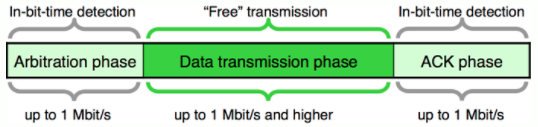
\includegraphics[width = \textwidth]{img/parts/introduction/CAN FD Bit Rates.png}
    \caption{Illustration of the \gls{can} FD flexible data-rate mechanism \citep{CANFD}}
    \label{fig:CANFD_BitRates}
\end{figure}

There exists also an extended version of \gls{can} FD, shown in Figure \ref{fig:CANFD_Extended}. It functions much like the classical extended \gls{can}, allowing for more IDs to be used.

\begin{figure}
    \centering
    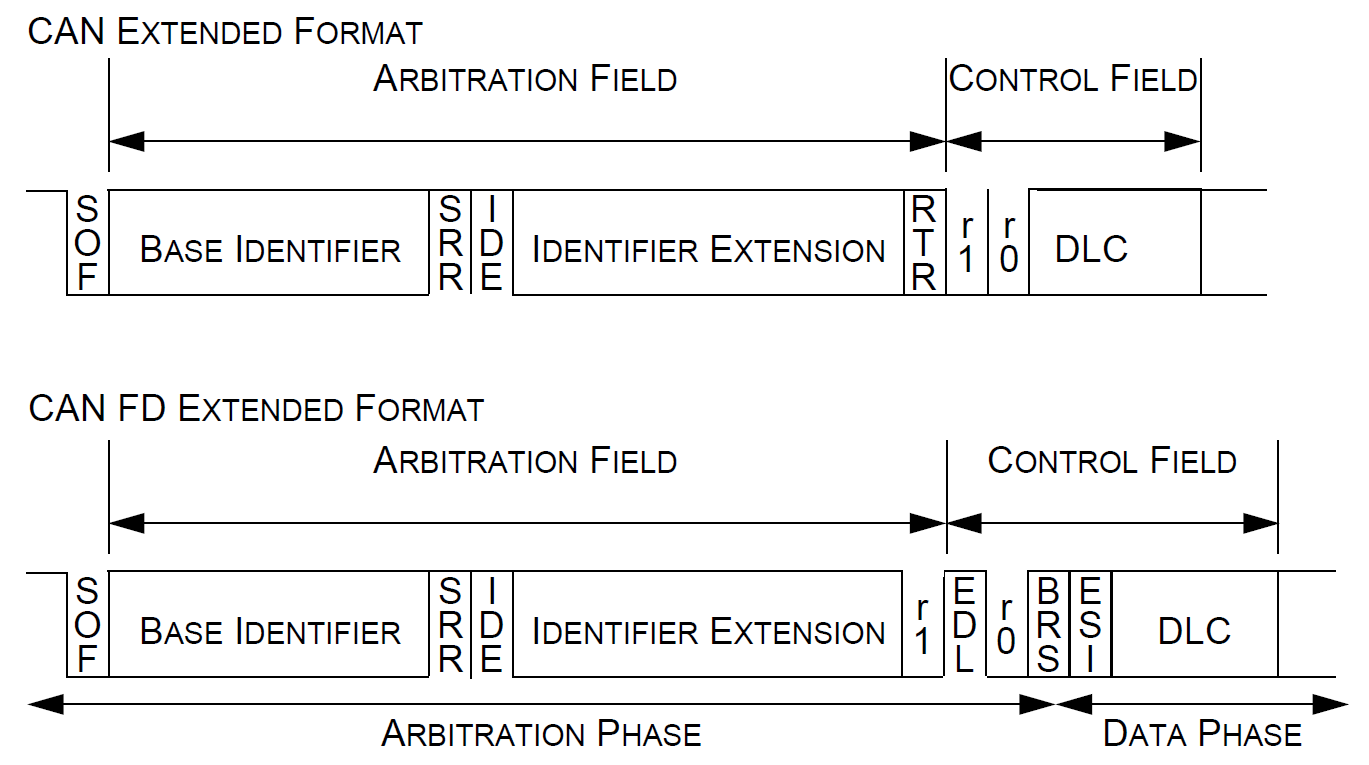
\includegraphics[width = \textwidth]{img/parts/introduction/CAN FD Extended.png}
    \caption{Comparison of extended \gls{can} and \gls{can} FD data frames \citep{Bosch2012}}
    \label{fig:CANFD_Extended}
\end{figure}

A major challenge in securing \gls{can} has been the limited speed and payload size, as it makes it difficult to implement typical cryptographic schemes, such as authentication, to defend against attacks. \gls{can} FD brings some relief in this matter, and new techniques have been proposed, like the ones in \citep{Woo2016} and \citep{Agrawal2019}.

\subsection{CAN XL}

Fueled by much of the same objectives as \gls{can} FD, as well as the rise in popularity of automotive Ethernet, \gls{can} XL presents itself as the third generation of \gls{can}, capable of providing speeds above 12Mb/s in the frame's data phase (the arbitration phase of the frame maintains its top bit-rate of 1Mb/s). This puts both 10BASE-T1s Ethernet and \gls{can} XL at the same level in terms of bit rate.\par

In contrast to 10BASE-T1s Ethernet, \gls{can} XL offers a wider range of topologies to choose from, meaning that not all \gls{can} XL networking topologies can be exactly replaced with Ethernet, as the latter has a stricter bus topology. An example of this can be seen in Figure \ref{fig:EthernetCANXL_Topologies}. The increase in data field length for \gls{can} XL also allows for transparent Ethernet frame tunnelling, enabling the use of IP communication \citep{BoschCANXL}. Another advantage this protocol has over automotive Ethernet is the fact that it is much easier to upgrade existing \gls{can} networks to \gls{can} XL than it is to transition to Ethernet and the IP stack, which is more complex and requires more expensive controllers \citep{VectorCANXL}. Seen as though \gls{can} XL can be mixed with \gls{can} FD, it also allows manufacturers to optimise cost by using the cheaper technology where higher bandwidth is not required \citep{BoschCANXL}.

\begin{figure}
    \centering
    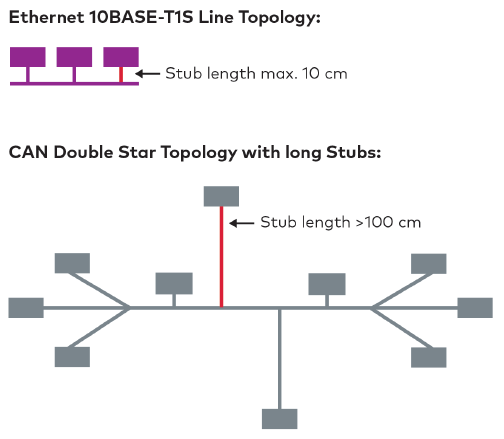
\includegraphics[width = \textwidth]{img/parts/introduction/Ethernet and CAN XL Topologies.png}
    \caption{Comparison between 10BASE-T1s and \gls{can} XL topology requirements \citep{VectorCANXL}}
    \label{fig:EthernetCANXL_Topologies}
\end{figure}

The \gls{can} XL frame structure can be seen in Figure \ref{fig:CANXL_Frame}.

\begin{figure}
    \centering
    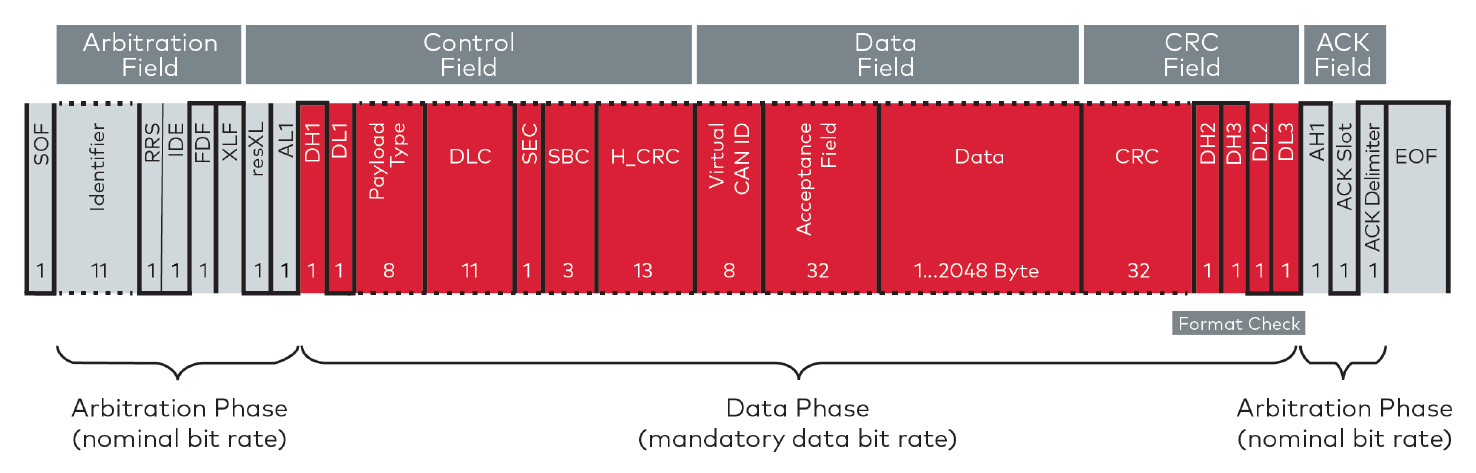
\includegraphics[width = \textwidth]{img/parts/introduction/CAN XL.png}
    \caption{Current status of development of the \gls{can} XL frame \citep{VectorCANXL}}
    \label{fig:CANXL_Frame}
\end{figure}

In Classical \gls{can} and \gls{can} FD, the \gls{can}-ID field (11 bit or 29 bit) is used for both arbitration and addressing purposes. In \gls{can} XL these functions are separated. The \gls{can} XL protocol separates the priority functions (11-bit Priority ID) and the addressing (32-bit AF). The 11-bit Priority Field provides the uniquely assigned priority of the \gls{can} XL DF. The 32-bit AF (Acceptance Field) is included in the 64-bit hardware acceptance filter of the \gls{can} XL controller. It may contain node address or content-indicating information.\par

The \gls{can} XL DF includes two CRC (cyclic redundancy check) fields: the 13-bit PCRC (Preamble CRC) in Control Field and the 32-bit FCRC (Frame CRC) in CRC Field. The CRCs are cascaded, which means the FCRC protects the whole frame, including the PCRC. Both CRCs can detect any five randomly distributed bit-errors, which corresponds to a Hamming distance of 6 \citep{CiACANXL}. New in the control field are also the possibilities to indicate the payload type, much like the EtherType field in Ethernet, and a virtual \gls{can} ID, allowing the separation of the \gls{can} network into virtual networks and comparable to the VLAN ID in Ethernet \citep{BoschCANXL}.\par

\gls{can} XL, therefore, presents itself as an incremental upgrade step for existing \gls{can} and \gls{can} FD networks, while also closing the gap in transmission speed between \gls{can} and automotive Ethernet. It aims to be a reliable alternative to 10BASE-T1s, with a simpler protocol stack and cheaper controllers. The fact that it allows for Ethernet frame tunnelling may also open the doors to joint single-based communication in the lower levels of the network (\gls{can}) and signal-based communication at the higher end (10BASE-T1s) \citep{VectorCANXL}.

\section{Automotive cybersecurity}

\subsection{Vulnerabilities}

\subsubsection{\gls{can}}

The reason \gls{can} is so dominant in the automotive networking space is because of its simplicity. This has, however, become an exploitable property with the exterior connectivity that did not exist when the protocol was developed.\par

Because messages are broadcast to the entire network, an attacker with access to one part of the network, like an ODB port, can eavesdrop on all traffic as well as send messages to all nodes. When eavesdropping, messages can be easily interpreted because there is no encryption in the protocol. There is also no authentication methods that allow nodes to know the source of the received frame, meaning that nodes cannot assert if a received frame was sent by a legitimate node or a bad actor. The ID-based arbitration scheme also facilitates Denial of Service attacks, as flooding the system with high-priority messages would cause all others to back off \citep{scalas2019automotive}.

\subsubsection{Wireless sensor networks}

Because of the wireless nature of the communication channel, messages can easily captured and replayed. Other problems with these communication protocols include the lack of proper cryptographic protection, the use of obscure code in the name of security, bad programming practices, and insufficient hardware protection against side channel attacks \citep{Le2018}.\par

\cite{rouf2010security} documented out several vulnerabilities of a \gls{tpms}, showing that its messages are both unencrypted and easily spoofed. They also showed that in-vehicle systems do not perform any input validation on incoming messages, and that it is highly possible to track vehicles through it.

\subsubsection{V2X communication}

Connecting a compromised device to a vehicle can result in attacks to in-vehicle systems. It's very common to connect a smartphone to a vehicle, either via Bluetooth or USB. Since smartphones can be infected with malware, in-vehicle applications must be protected it. \cite{mirrorlink}, for example, trusts all contents from registered smartphones, which may be infected \citep{mazloom2016security}. Other equipment for V2V and V2I communication can also be exploited via a bad implementation or configuration.

\subsection{Common attack patterns}

The authors of \cite{Kim2021} surveyed previously published research on attacks against autonomous vehicles, although some attacks are also effective against non-autonomous vehicles. They classify attack research into three categories: attacks on the automotive control system, attacks on the autonomous driving system components, more specifically through mobile apps, and attacks on Vehicle-to-Everything (V2X) communication technologies.

\subsubsection{Automotive control systems}

One type of automotive control system attack targets the vehicle’s \glspl{ecu}. Taking advantage of network vulnerabilities, research shows that it is possible to load firmware into \glspl{ecu} that control components such as the door-lock and telematics, primarily through fuzzing \citep{Koscher2010}. The vulnerabilities described by \cite{rouf2010security} showed that it is possible for an attacker to remotely display a false tire pressure warning or disable the \gls{tpms} \gls{ecu}, as well as vehicle tracking from 10-40 metres. More recently, it was shown that \glspl{ecu} present in Tesla vehicles could be controlled remotely by sending arbitrary \gls{can} packets, which led Tesla to introduce code-signing protection in an Over-The-Air (OTA) update \citep{Nie2017}. \cite{miller2015remote} showed that, even remotely, and attacker can reprogram \glspl{ecu}, control display and sound systems, the instrument cluster, body components, interfere with the engine operation, lock and disable brakes, prevent the car from turning on or off, etc. They showed that, even from telematics \glspl{ecu}, this type of attack has the same effects as directly injecting messages into \gls{can} buses.\par

In-vehicle network attacks aim to disrupt communication between vehicle components. In \citep{Palanca2017}, the authors showed that the \gls{can} bus is vulnerable to selective \gls{dos} attacks, which cannot be detected at the frame level. Sniffing and replay attacks have also been demonstrated, as per \cite{hoppe2009applying}. \cite{nilsson2009first} also explored possible attacks on the FlexRay protocol. They showed that, because there is no encryption, it is possible to read all data sent to the bus, as well as insert unauthenticated messages. A successful attack causes serious disruption of the vehicle control system and may harm drivers and passengers.\par

Passive key-less entry and start systems used in modern cars are a major attack target. It has been shown that some systems are vulnerable to relay attacks by duplicating the existing signal \citep{francillon2011relay}. Through the analysis of cryptographic vulnerabilities, \cite{verdult2012gone} demonstrated how private keys could be recovered from the Hitag2 transponder in order to bypass the key's cryptographic authentication in as little as 6 minutes. \cite{garcia2016lock} also showed how to recover cryptographic keys and clone a VW group remote via eavesdropping on a single signal, as well as another Hitag2 attack able to clone the remote in just a few minutes.\par

\subsubsection{External communication technologies}

A comprehensive survey of attacks on \glspl{vanet} \cite{Hasrouny2017} showed that these are vulnerable to the same attacks as a regular network, such as \gls{dos}, man in the middle, message suppression, or spoofing.\par

The integration of Bluetooth has become standard, and it brings with it a new set of vulnerabilities. In \cite{Cheah2017}, it was shown that manufacturers still include the ability to use legacy pairing, which led the authors to identify vulnerabilities. Other research has shown the execution of attacks using Bluetooth as a vulnerable component, as shown in \cite{Cai2019} with BMW cars.

\subsubsection{Mobile apps}

The increase in connectivity between the driver’s vehicle and his smartphone led to an expansion in the vehicle’s attack surface. A malicious smartphone app could be used to gain unauthorised access to a vehicle without needing to be in its proximity (i.e., using long-range wireless networks). The authors of \cite{Woo2015} exploited \gls{can} vulnerabilities in the process of demonstrating this scenario. Vulnerabilities in the MirrorLink protocol have also allowed attackers to send \gls{can} packets through a smartphone, opening the possibility for a variety of exploits. The attack method present in \cite{mazloom2016security} took advantage of a heap overflow. A vulnerability in Blue Link, a vehicle control application from Hyundai Motors, allowed the recovery of the driver's username, password, and PIN. An attacker could also exploit this vulnerability to remotely unlock the vehicle \citep{toddbluelink}. With the smartphone being relatively vulnerable to attacks, and with manufacturers providing more functionality to it's connection to the vehicle, it is expected that these type of applications become a major target \citep{Kim2021}.

\subsection{Proposed solutions}

The development of protection mechanisms faces multiple constraints resulting from the limited computing resources available to each \gls{ecu} as well as the time-sensitive nature of their operations. There is also a need to assert retro-compatibility with currently used embedded technologies, and, when considering external entities, interoperability between their security mechanisms. Two distinct vehicles, for example, should not be prevented from communicating because their protocols are incompatible \citep{Studnia2013}.\par

There is an effort by European projects such as Secure Vehicular Communication (SeVeCom) \citep{Kargl2008}, Preparing Secure Vehicle-to-X Communication Systems (PRESERVE) \citep{PRESERVE}, or E-safety Vehicle Intrusion Protected Applications (EVITA) \citep{EVITA}, to design secure vehicle communication architectures.\par

For \glspl{vanet}, the usage of public-key infrastructure has also been proposed, to assert the authenticity of the messages, as well as the use of pseudo-anonymity to preserve privacy. For preventing \gls{dos} attacks, some routing protocols have also been studied \citep{Hasrouny2017}.\par

Regarding internal protection, there have been several attempts to leverage cryptography in securing the \gls{ecu} and the \gls{can} bus. An authentication protocol, such as the one proposed in \citep{Herrewege2011} or \citep{Groza2018}, would prevent most injection attacks. Another approach, taken by the EVITA project, consists in the implementation of a dedicated hardware module for cryptographic operations \citep{Wolf2011}.\par

\gls{ids} has traditionally been used in network security, more specifically in desktop IT. \citep{hoppe2009applying} is one of the first to mention its usage in automotive IT as a “promising supplemental measure”. They also discuss a way to optimally communicate a warning to the driver.

\section{Machine learning}

As stated in \ref{sec:ids_detection_approaches}, the use of machine learning in an \gls{ids} allows it to adapt and detect previously unseen attacks. Such an approach has two phases: training and testing. First, attributes and classes from the training data must be identified. These must be reduced to a subset of those most relevant for classification, discarding unnecessary ones (\textit{i.e.}, dimensionality reduction). Then, the resulting dataset is used to train the model, with the trained model being used to classify unknown data. The training data can be unlabelled, which creates an unsupervised learning problem, partially labelled, for semi-supervised learning, or fully labelled, making the learning phase supervised \citep{Buczak2016}.\par

In \citep{Shearer2000}, the CRoss Industry Standard Process for Data Mining (CRISP-DM) was presented as a six-phase model describing the data science life cycle in a industry, tool, and application neutral way. A representation of this can be see in Figure \ref{fig:CRISP-DM}.

\begin{figure}
    \centering
    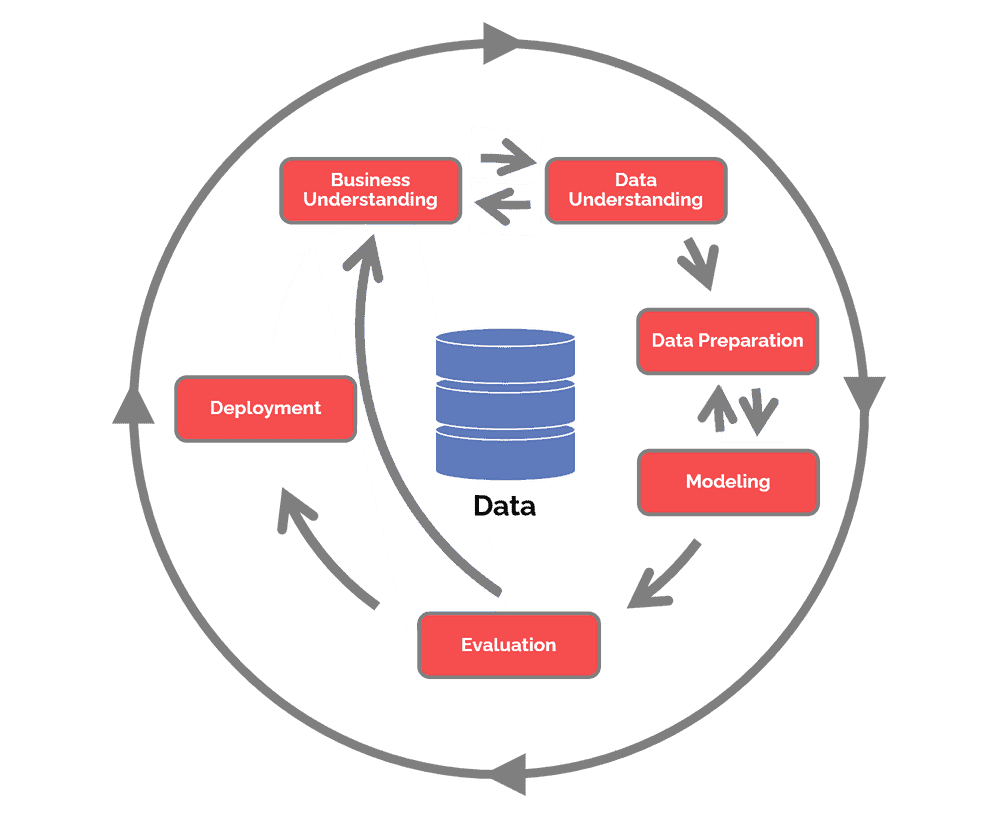
\includegraphics[width = .7\textwidth]{img/parts/introduction/CRISP-DM.png}
    \caption{CRISP-DM diagram \citep{DSPA}}
    \label{fig:CRISP-DM}
\end{figure}

The model's six phases are:
\begin{itemize}
    \item Business understanding, where the project's requirements are defined.
    \item Data understanding, where data is collected and examined.
    \item Data preparation, where the collected data is processed to produce the final dataset.
    \item Modeling, where machine learning methods are applied to produce the model.
    \item Evaluation, to verify whether the produced model is able to verify the requirements established in the first phase.
    \item Deployment, with the model being implemented.
\end{itemize}

In most applications, machine learning models are trained and then used for a long time without any modifications. In the security space, however, new threats emerge frequently. This means that models must be updated often in order to learn to detect new and emerging attack, as well as in cases where the network traffic suffers modifications in its usual pattern. Training times are, therefore, important. The model's ability to learn incrementally is also valuable, as training from scratch every time new data appears would be very time consuming.\par

Network traffic also generates a huge amount of unlabelled data, and labelling it is a laborious task. Quickly acquiring novel attack data can also be difficult, but is necessary to update the model as soon as possible \citep{Buczak2016}.\par

Deep learning is a subset of machine learning where the neural networks have more than one hidden layer. While machine learning algorithms make use of labelled and structured data to make predictions, deep learning algorithms automate feature extraction and can ingest and process unstructured data \citep{ibmDeepLearning}.

\subsection{Performance metrics}

There are several metrics used to classify a model's performance. To access if the model will generalise to an independent dataset, cross validation techniques are commonly used. Cross validation consists of a re-sampling method that iterates several times over a given dataset, sampling distinct training and test sets each time. This is particularly useful if the amount of available data is small.\par

For binary classification tasks, the confusion matrix provides several useful performance metrics by laying out true and false positives, as well as true and false negatives in a 2x2 table. Many relevant metrics can be inferred from these values, as shown in Figure \ref{fig:confusion_matrix}. The true-positive rate, also known as recall or sensitivity, provides the rate at which the model detects a truly positive case, while the false-negative rate is the proportion of positive cases missed. The false-positive rate is the probability of the model classifying a negative case as positive, and the true-negative gives the rate at which the model correctly identifies negative cases. Prevalence is the proportion of the dataset that is actually positive, while accuracy tells us how many correct predictions (both positive and negative) the model made in proportion to the total dataset. The positive predictive value metric, or precision, represents the likelihood that a positive prediction is actually positive, with the false discovery rate being its complement. The negative predictive value and false omission rate are analogous. The positive and negative likelihood ratios tell the probability that a classification is actually positive or negative is the model classifies it at such. The diagnostic odds ratio provides a way to measure the model's performance without, unlike accuracy, being affected by prevalence. The F1 score is a function of both precision and recall to give an overall indication of the classifier's performance.

\begin{figure}
    \centering
    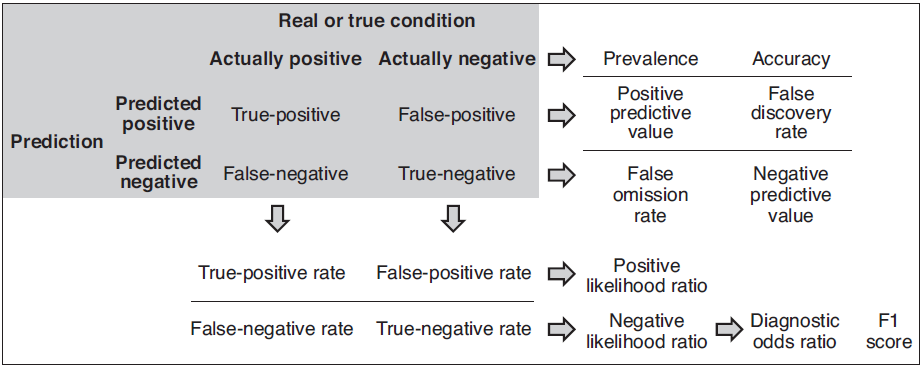
\includegraphics[width = .7\textwidth]{img/parts/introduction/Confusion Matrix.png}
    \caption{Components of a confusion matrix \citep{Handelman2019}}
    \label{fig:confusion_matrix}
\end{figure}

Another widely used metric for evaluating performance in binary classification tasks is the area under the receiver operating characteristic curve (AUROC). The curve is a graphical plot that illustrates the true-positive versus false-positive rates as the discrimination threshold is varied. A variation in the discrimination threshold usually means a gain in one metric, but a loss in the other, \textit{e.g.} a higher threshold value will decrease the classifier's recall, but increase its precision, and vice-versa. Good performing classifiers will have a large area under the plotted curve.\par

For regression problems, the mean squared error (MSE) is generally used as a way to evaluate how good the model's predictions are (\textit{i.e.}, how close they are to the true value). The MSE is calculated as the mean or average of the squared differences between predicted and expected target values in a dataset, where a lower value is preferred. The rooted mean square error (RMSE) is an extension of the MSE where the units of the metric are the same as the units of the target value (and not its square). The mean absolute error, unlike MSE and RMSE, does not punish large error values as harshly as the other two metrics, as its value increases linearly with the error size, and not quadratically. The coefficient of determination ($R^2$) indicates how much of the observed variations in the data are explained by the model, in which case a higher value is better \citep{Handelman2019, Brownlee2021}.

\subsection{Datasets}

Both the size and quality of the dataset are very important to achieve good model performance. For networking purposes, there are different types of data, with the most common being packet capture data and NetFlow.\par

Packet capture data consists of data captured by the networking interface, at the packet level. NetFlow is a router feature introduced by Cisco, giving it the ability to collect IP network traffic that goes through the interface, identifying packet flow. NetFlow version 5 defines a network flow as a unidirectional sequence of packets that share the exact same seven packet attributes: ingress interface, source IP address, destination IP address, IP protocol, source port, destination port, and IP type of service \citep{Handelman2019}. Table \ref{tab:network_datasets} shows a comparison between several public datasets.

\begin{table}
    \centering
    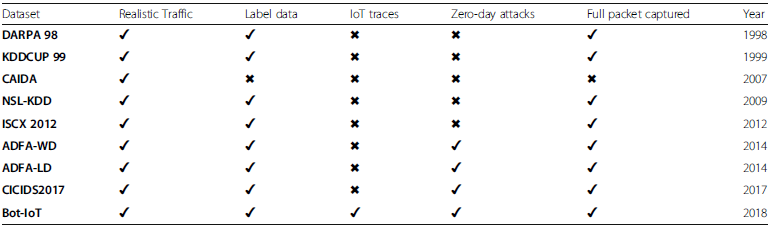
\includegraphics[width = \textwidth]{img/parts/introduction/Network Datasets.png}
    \caption{Comparison of network traffic datasets \citep{Khraisat2019}}
    \label{tab:network_datasets}
\end{table}

A majority of the effort in compiling networking datasets has been placed in the real of IP networks. In the automotive domain, there is a clear lack of such comprehensive datasets, especially when looking for labelled datasets containing attacks. Some datasets commonly used in \gls{ids} research for \gls{can} are \cite{CANDataset_OTIDS, CANDataset_Car-Hacking, CANDataset_TUE, CANDataset_IEEE}.

\subsection{Machine learning techniques}
\label{subsec:machine_learning_techniques}

\subsubsection{Supervised learning}

\paragraph{Decision trees}
A decision tree is a flowchart-like structure with three basic components: a decision node, containing the test attribute, a branch, containing a possible decision based on the attribute, and a leaf, identifying the class that the instance belongs to. The best known algorithms for constructing decision trees are the ID3 and the C4.5 algorithms \citep{Badr2014, Buczak2016}.

\paragraph{Naïve Bayes}
This technique applies Bayes' principle with assumptions that the input features are independent. It is an optimal classifier if the features are conditionally independent, although this is rarely true. One of its biggest advantages is that training can be completed in linear time \citep{Buczak2016}. The Hidden Naïve Bayes model is more sophisticated and can be applied to highly dimensional \gls{ids} tasks, with interrelated attributes and high-speed networks \citep{Khraisat2019}.

\paragraph{Evolutionary computation}
An evolutionary computation algorithm is based on the \emph{survival of the fittest} principle. Starting with a randomly generated population, a fitness value is computed for each individual from the population, revealing how good it is at solving a given problem. Fitter individuals are copied into the next generation, and the process continues. The two most widely used methods are Genetic Algorithms (GA) and Genetic Programming (GP). In GA, individuals are represented as a series of bits, to which selection and reproduction operators are applied favouring fitter solutions. In GP, individuals are represented as programs with operators (\textit{e.g.} plus, minus, and, or) and programming blocks (\textit{e.g.} if, while), and crossover and mutation operations are more complex than those in GA.

\paragraph{Artificial neural network}
The mechanisms behind an artificial neural network are similar to those of a brain. Input data is fed to a first layer of neurons, where a computation is performed and the output is fed to the next layer of neurons. The result is the output of the last layer. The model learns by looking at the error between the output and the desired outcome, and adjusting the computations, typically through backpropagation methods. For IDSs, the frequency of certain attacks in the dataset impacts how well it will be recognised, making it difficult for the model to recognise less frequent attacks \citep{Khraisat2019}.

\paragraph{Fuzzy logic}
Unlike in conventional boolean logic, where there are only true or false values, fuzzy logic allows an instance to partially belong to multiple classes at the same time, allowing for degrees of uncertainty. This makes it a good classifier for an \gls{ids}, where the border between normal and abnormal behaviour is not well defined and, therefore, reducing the rate of false alarms \citep{Khraisat2019}.

\paragraph{Support vector machines}
This classifier works by finding a hyperplane in the feature space that separates two classes so that the distance between the hyperplane and the closest data points is maximised. This is a favourable method in situations where the number of features is much greater than the number of data points \citep{Buczak2016}.

\paragraph{Hidden Markov model}
A Markov process is a stochastic model describing a sequence of states where the probability of transitioning to any particular state is dependent solely on the current state and time elapsed \citep{Maltby}. An Hidden Markov model is a statistical Markov model where the modelled system is assumed to be a Markov process with unseen data, where its states represent unobservable conditions \citep{Buczak2016}.

\paragraph{K-nearest neighbours}
The idea behind this method is to classify a point based on the $k$ nearest samples, where $k$ is the number of samples being considered. Majority voting is used to determine the classification, which can be a pitfall if the class distribution is skewed \citep{Buczak2016}.

\paragraph{Recurrent Neural Networks}
A \gls{rnn} is a feed-forward deep learning neural network in which each unit bases its decision making process on its current input and the output of the previous input. It is widely used in natural language processing and speech recognition \citep{ibmDeepLearning}. Although it can only handle limited length sequences and may suffer from short-term memory if the input length is too long, \gls{rnn} variants like \gls{lstm} and \gls{gru} have been developed to solve these issues \citep{ahmad2021network}.

\paragraph{Deep Neural Network}
A \gls{dnn} is a deep learning structure composed of an input layer, many hidden layers, and an output layer. Increasing the number of hidden layers improves the model's abstraction level, and its used to model complex nonlinear functions \cite{ahmad2021network}.

\paragraph{Deep Belief Network}
A \gls{dbn} as a deep learning model composed of stacked \gls{rbm} (a two-layer model with data flowing in both directions) in layers followed by a softmax classification layer. In a \gls{dbn}, connections exist between the layers but not between units within each layer \cite{ahmad2021network}.

\paragraph{Convolutional Neural Network}
\glspl{cnn} have three main types of layers: convolutional layer, pooling layer, and fully-connected layer. The convolutional layer is the first layer of a convolutional network. While convolutional layers can be followed by additional convolutional layers or pooling layers, the fully-connected layer is the final layer. With each layer, the network increases in its complexity, identifying greater portions of the input data. Earlier layers focus on simple features, and data progresses through the layers of the CNN, it starts to recognise larger patterns \cite{ibmCNN}.

\subsubsection{Unsupervised learning}

\paragraph{Clustering}
This is an unsupervised pattern discovery approach which groups unlabelled data based on their similarities or differences. Clustering algorithms can be exclusive, overlapping, hierarchical, and probabilistic \citep{IBM}. In exclusive clustering, a data point can exist be a part of no more than one cluster. K-means clustering is an example of an exclusive clustering algorithm, where the aim is to separate data objects into $k$ clusters, where each observation belongs to the cluster with the nearest mean. On the other hand, overlapping clustering allows a data point to be a part of multiple clusters at once (\textit{e.g.} fuzzy k-means). Hierarchical clustering seeks to create a hierarchy of clusters, and the approach can be categorised in two ways: agglomerative, which is a bottom up approach where sub-clusters are grouped together as one moves up through the hierarchy, and divisive, where the largest cluster in diameter is separated into sub-clusters \citep{Khraisat2019}. Probabilistic clustering, data points are clustered based on the likelihood that they belong to a particular distribution, with the Gaussian Mixture model being commonly used \citep{IBM}.

\paragraph{Association rules}
An association rule describes a relationship among different attributes: \emph{if (A and B) then C}, with metrics revealing how often a given relationship occurs in the data. Fuzzy association rules extend this functionality into categorical or quantitative data, instead of boolean only. These take the form of \emph{if (X is A) then (Y is B)} \citep{Buczak2016}.

\subsubsection{Statistical inference}

\paragraph{Inductive learning}
This method attempts to find patterns and regularities in the observations, and then makes general conclusions or theories about the data in the form of rules.
% RIPPER

% \subsubsection{Ensemble}

\subsection{Support Vector Machines}

As stated in \ref{subsec:machine_learning_techniques}, \glspl{svm} are a supervised machine learning model for non-probabilistic binary classification (although methods such as Platt scaling allow for it's use in a probabilistic classification setting \citep{platt1999}) through the construction of one or several hyperplanes that best separate data into distinct categories. This classifier works by mapping the input space into a higher-dimensional feature space, where separation between classes becomes easier, and finding a hyperplane that separates two classes so that the distance between the hyperplane and the closest data points is maximised \citep{Buczak2016}. New data is then classified based on their positioning relative to those hyperplanes. An example of this can be seen in Figure \ref{fig:svm_hyperplane}.

\begin{figure}
    \centering
    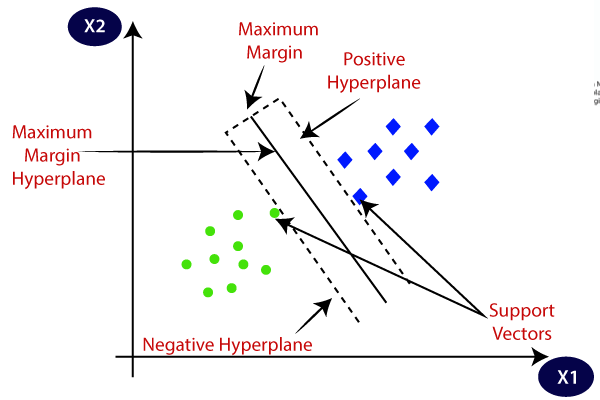
\includegraphics[width = \textwidth]{img/parts/app/Support Vector Machine.png}
    \caption{A hyperplane separating two classes \citep{JavaTpoint_SVM}}
    \label{fig:svm_hyperplane}
\end{figure}

Mapping the input space into the feature space is done through an approach called the "kernel trick". This allows the algorithm to operate in the feature space without the need to map each data point into a higher dimension, which is computationally expensive. Instead, a kernel method is more efficient by using only the dot product of all pairs of data to achieve this same effect. Popular kernels include the linear, polynomial, and Gaussian (or radial basis function) kernels:

\begin{itemize}
    \item Linear: $K(x, y) = x^Ty$
    \item Polynomial: $K(x, y) = (x^Ty + c)^d$, where $c>=0$  is a parameter that trades off the influence of higher-order against lower-order terms in the polynomial, and $d$ is the polynomial degree.
    \item Radial basis function: $exp(-\frac{\Vert x - y \Vert ^2}{2\sigma^2})$, where $\sigma$ is a free parameter.
    \item Sigmoid (hyperbolic tangent): $K(x, y) = tanh(\alpha x^Ty + c)$, where $\alpha$ is the slope and $c$ a constant.
\end{itemize}

The Gaussian kernel consistently reports good results in practical situations, but is computationally more expensive than the linear or polynomial alternatives \citep{bounsiar2014one}.\par

\cite{scholkopf1999} then introduced an "extension to the support vector algorithm" adequate for novelty detection through unsupervised learning. Here, data is not classified as belonging to one of two classes, but as belonging to one class or everything else (hence the name). It has become one of the most popular methods for anomaly detection. Training is done on using only positive (normal) data, which is advantageous since anomalous data can be difficult to obtain when comparing to the large amount of normal data that can be easily obtained from most systems. This algorithm has been successfully used in a variety of domains, such as \cite{tian2018ramp, miao2018distributed, amraee2018abnormal}.\par

The \gls{ocsvm} algorithm attempts to create a decision boundary that provides the maximum separation between the training data points and the origin, with only a fraction of data points being allowed to reside outside of the decision boundary. To do this, the origin is treated as the only member of the non-target class.\par

The primary objective function of the \gls{ocsvm} is

\begin{gather*}
\min_{e, \xi, \rho} \frac{\Vert \omega \Vert ^2}{2} - \rho + \frac{1}{\nu n} \sum_{i=1}^{n} \xi i \\ \text{subject to: } w^T \phi (x_i) \geq \rho - \xi_i \wedge \xi_i \geq 0
\end{gather*}

\noindent
where $\xi_i$ is the slack variable that allows certain points to reside outside the boundary (in order to avoid over-fitting), $\omega$ is the vector perpendicular to the decision boundary, $\phi(\cdot)$ is the nonlinear transformation that maps samples to the high-dimensional feature space, $\rho$ is the distance to the origin, $n$ is the training set size, and $\nu$ is the regularisation parameter which describes the trade-off between over-fitting and generalisation by setting an upper-bound on the fraction of outliers and a lower-bound on the number of support vectors.\par

Using Lagrange multipliers and a kernel function for dot product calculations, to avoid the computation of the nonlinear mapping, the decision function becomes

\begin{gather*}
\min_{\alpha}\left\{\frac{1}{2} \sum_{i, j} \alpha_i \alpha_j K(x, y)\right\}\\
\text{subject to: } 0 \leq \alpha_i \leq \frac{1}{\nu n} \wedge \sum_i \alpha_i = 1
\end{gather*}

\noindent
which, after solving the dual problem and obtaining a set of model weights $\alpha_i$, provides the decision function for any test vector $z_*$:

\[
f(z_*) = \text{sgn} \left( \sum_i \alpha_i K(x, z_*) - \rho \right)
\]

\subsection{Time complexity}

The amount of time it takes to run an algorithm dictates whether it can be trained in an online fashion or not. Algorithms that take a long time to process data can easily be overwhelmed by a streaming input, potentially bottlenecking network throughput.\par

Time complexity is typically expressed using big O notation (\textit{e.g.} $O(n)$, $O(n\ log\ n)$, $O(n^2)$), where n is the size in units of bits needed to represent the input. \citep{Buczak2016} state that, as a rule of thumb, the $O(n)$ and $O(n\ log\ n)$ algorithms are considered to be linear time and are usable for online approaches. $O(n^2)$ is considered as acceptable for most practices. $O(n^3)$ and higher are considered to be much slower algorithms and used for offline approaches. Table \ref{tab:algo_comparison} shows a comparison between different algorithms, assuming $n$ to be much larger than $m$. Most machine learning methods have linear time complexity on the testing phase, and can, therefore, be used online.

\begin{table}
    \centering
    \begin{tabular}{*{4}{|m{.2\textwidth}}|}
    
    \hline
    \textbf{Algorithm} & \textbf{Typical Time Complexity} & \textbf{Streaming Capable} & \textbf{Comments}\\
    \hline\hline
    
    Artificial Neural Network & O($emnk$) & low & $e$: number of epochs\newline $k$: number of neurons\\
    \hline
    Association Rules & >>O($n^2$) & low &\\
    \hline
    Bayesian Network & >>O($mn$) & high &\\
    \hline
    Clustering, k-means & O($kmni$) & high & $i$: number of iterations until threshold is reached\newline $k$: number of clusters\\
    \hline
    Clustering, hiearchical & O($n^3$) & low &\\
    \hline
    Clustering, DBSCAN & O($n \log n$) & high &\\
    \hline
    Decision Trees & O($mn^2$) & medium &\\
    \hline
    GA & O($gkmn$) & medium & $g$: number of generations\newline $k$: population size\\
    \hline
    Nearest Neighbour k-NN & O($n \log k$) & high & $k$: number of neighbours\\
    \hline
    \end{tabular}
    \caption{Complexity comparison of machine learning algorithms during training \citep{Buczak2016}}
    \label{tab:algo_comparison}
\end{table}

\begin{table}
    \centering
    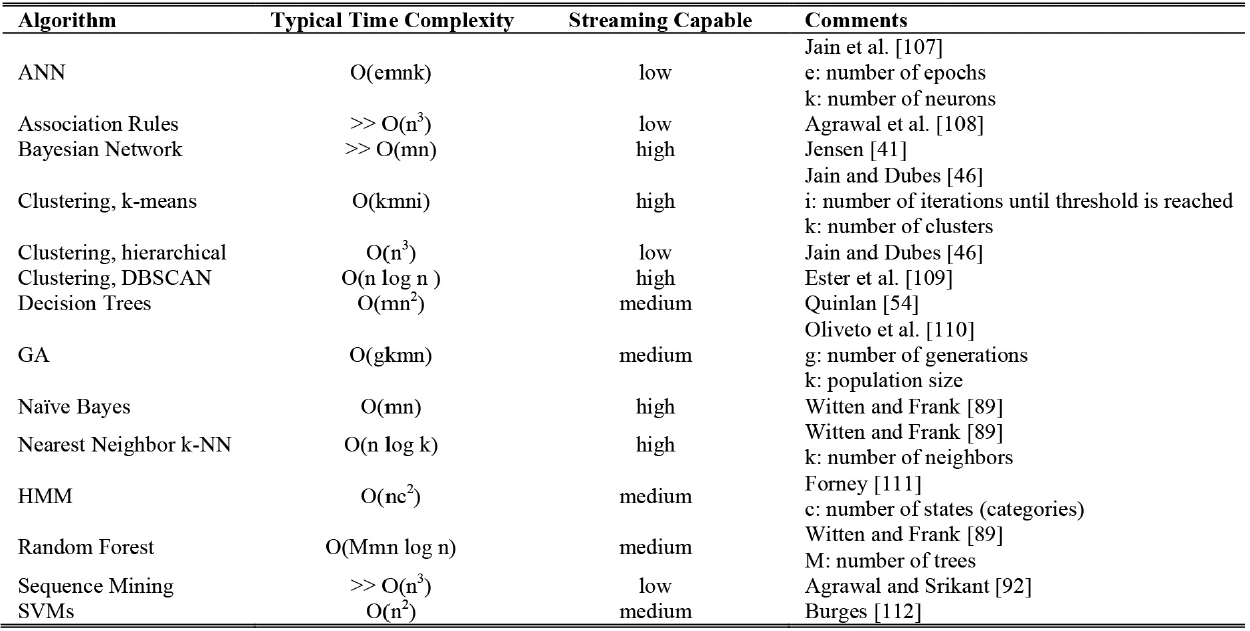
\includegraphics[width = \textwidth]{img/parts/introduction/Algorithm Comparison.png}
\end{table}

\subsection{Anomaly detection}

Novelty detection, also known as semi-supervised anomaly detection \citep{Scikit-learn-novelty_detection}, is the task of recognising data in the test set that differs in some respect to the data available during training. It is particularly useful when there is a large amount of "normal" data, but insufficient "abnormal" data. This is common in settings where measurements of a normal operating state are inexpensive to obtain, but generating a large amount of data in abnormal states is both difficult and costly. The goal is to train a model with what is considered to be "normal" data and then use that model to detect anomalies, \textit{i.e.} data not present in the training set. The techniques used should have a high detection rate, but with few false alarms, be scalable, and good time and space complexity. \cite{pimentel2014review} classified anomaly detection techniques into five categories: probabilistic, distance-based, reconstruction-based, domain-based, and information-theoretic.

\subsubsection{Probabilistic methods}

This approach is based on estimating the generative probability density function of the data, which is then thresholded in order to determine if a test sample originated from the same distribution or not. The estimation of the underlying data density from multivariate training data falls under two categories: parametric and non-parametric.\par

Parametric statistics assumes that the distribution of the population is known and is based on a fixed set of parameters \citep{IBM_ParatericStatistics}. The Gaussian distribution is commonly used for continuous variables, but more complex distributions may use mixture models such as \gls{gmm}. State-space models, often used in time-series data, assume that there are unobserved variables or parameters (states) that describe the evolution of the underlying system. Common state-space models used for novelty detection are the \gls{hmm} and the Kalman filter.\par

Non-parametric statistics makes no assumptions about the population's distribution or it's parameters. The use of kernel density estimators is an approach in which the probability density function is estimated using a large number of kernels distributed over the data space (\textit{e.g.} the Gaussian kernel).\par

Probabilistic methods are a mathematically well-grounded, effective, and transparent way to identify novel data as long as an accurate estimate of the data's probability density function has been obtained. However, this performance is limited when the training set is small. Non parametric approaches are usually preferred because prior knowledge of the data's distribution parameters is typically unavailable.

\subsubsection{Distance-based methods}

These methods determine the similarity between two observations based on distance metrics. Most methods are $k$-nearest neighbour- or clustering-based.\par

The $k$-nearest neighbours is a supervised algorithm that assumes that normal data points are close to each other, while anomalies are located far from these points. The Euclidean distance is a popular choice for distance measurement, and local density, in which the average of the $k$ nearest neighbours is considered, determines if a point is an anomaly or not.\par

The $k$-means clustering algorithm, a unsupervised algorithm, is a clustering-based method for identifying abnormalities. Here, data points from the training set are divided into clusters and classifying data points based on the cluster into which they are inserted.\par

Both $k$-nearest neighbours and clustering algorithms rely on the existence of a suitable distance metric to detect anomalies. Although they are very effective at this task, they do not scale very well to high dimensional datasets.

\subsubsection{Reconstruction-based methods}

Reconstruction methods attempt to model the underlying training data and classify the testing data based on it's reconstruction error. Both neural networks and subspace-based methods can be trained this way.

\subsubsection{Domain-based methods}

Domain-based methods attempt to define a boundary based on the training data, and testing samples are labelled based on their position relative to the boundary. \glspl{svm}, for example, generate a hyperplane that maximises the minimum distance to the closest point of either of the two classes. As for novelty detection, \glspl{svm} have been used in one of two ways: through the one-class approach, or through the support vector data description approach.\par

The aim of the one-class approach, introduced by \cite{scholkopf1999}, is to, though a kernel, separate all the data points from the origin and maximise the distance from this hyperplane to the origin. This does, however, require that a hyper-parameter corresponding to the percentage of data in the training set that is allowed to fall outside of this boundary.\par

The support vector data description method, proposed by \cite{tax2004} gives the training data a spherically shaped boundary with the minimum volume that encloses all, or most, of the data.\par

Although they are commonly used for anomaly detection, showing good performance, the kernel methods used can be computationally intensive. The choice of the appropriate kernel is also a challenge.

\subsubsection{Information-theoretic methods}

These methods attempt to detect novelties through significant changes in the information content of the data. Typical metrics include entropy, relative entropy, information gain, etc.